
\documentclass{jotarticle}
\title{URDAD for System Design}
%---------------------------------------------------------------------
% [AUTHOR] Add the authors here
%          Several authors can be separated by either \\ or \and
%          Use bold font for the authors name as shown in the example.
%---------------------------------------------------------------------
\author{Friedemann (Fritz) Solms \\ Solms Training, Consulting and Development\\ 
        113 Barry Hertzog Ave, Emmarentia, 2195, South Africa}
%---------------------------------------------------------------------


%---------------------------------------------------------------------
% CONFIGURATION: BY THE JOT TEAM
%---------------------------------------------------------------------
% [JOT] Set first page and last page of the article/column
%-----------------------------------------------------------Julian Israelsohn---------- 
\firstpage{1}
\lastpage{3}
%---------------------------------------------------------------------
% [JOT] Enter the volume and number of the issue. 
%       Here: vol 2, no 3
%---------------------------------------------------------------------
\jotvolume{2}
\jotnumber{2}
%---------------------------------------------------------------------
% [JOT] Enter the month and year when the issues is published.
%       Here: March 2003
%---------------------------------------------------------------------
\jotmonth{3}
\jotyear{2003}
%---------------------------------------------------------------------
% [JOT] [OPTIONAL] Enter how to cite this article 
%       This is generated. In case it does not fit your expectations,
%       you can enter it yourself.
%---------------------------------------------------------------------
\howtocite{\href{http://www.jot.fm/general/JOT_template_LaTeX.tgz}%
{http://www.jot.fm/general/JOT\_template\_LaTeX.tgz}}
%---------------------------------------------------------------------
% [JOT] Set type of paper, i.e. column or article
%       This is needed for the generation of \howtocite
%---------------------------------------------------------------------
\papertype{document}
%---------------------------------------------------------------------
% [JOT] Set the filename. 
%       This is needed for the generation of \howtocite
%---------------------------------------------------------------------
\filename{}
%---------------------------------------------------------------------
% [JOT] Enter the names of the authors as comma-separated list.
%       This is needed for the generation of \howtocite.
%       (I know this is ugly -- I will work on that as soon as type
%       permits it.) 
%---------------------------------------------------------------------
\authornames{Friedemann (Fritz) Solms}
%---------------------------------------------------------------------


%---------------------------------------------------------------------
% START OF THE DOCUMENT
%---------------------------------------------------------------------
% This is where the document starts. In this example, I will guide
% you through this sample article with the explanation of possible
% commands you should use.
%---------------------------------------------------------------------


%---------------------------------------------------------------------
\begin{document}
%---------------------------------------------------------------------

%---------------------------------------------------------------------
% ABSTRACT
%---------------------------------------------------------------------
% [AUTHOR] Clearly a job for the author :-)
%          Add your abstract here
%---------------------------------------------------------------------
\begin{abstract}
URDAD, Use-Case, Responsibility Driven Analysis and Design, provides a simple, intuitive design process which can be embedded within iterative, use-case driven software development methodologies like extreme programming or the Rational Unified Process (RUP). URDAD has been formulated in a way which encourages sound design principles. The process directly generates clean layers of granularity, with good responsibility localization across loosely components of minimal structural complexity. The resultant design is architecture and technology neutral. Following OMG's Model Driven Architecture (MDA) this platform independent design is mapped onto some choice of architecture and realization techonologies.
\end{abstract}

\section{Introduction}
\label{secIntroduction}

Good design makes systems more flexible and robust, reduces maintenance cost and increases life expectancy. Yet, generating a ``{\em good design}'' is a non-trivial task. This article looks at core attributes of good design and explains how URDAD provides a simple algorithmic design process which leads to a design satisfying many of the requirements of a good design.

\subsection{Design versus development processes}
\label{secDesignVersusDevelopmentProcess}

Software developers are phased with the problem of having to provide a design and ultimately an implementation which realizes the use case requirements. Software development processes like RUP (the Rational Unified Process) and Extreme Programming provide a higher level process for effectively managing the risk and quality of the development process. They do not, however, provide a design process. One still has to decide how to design and integrate the system components in order to obtain the desired functionality.

URDAD addresses this problem by providing a process for taking a use case through to realization processes.

\subsection{Background}
\label{secBackground}

URDAD has grown out of Responsibility Driven Design (RDD) methodology pioneered by Rebecca Wirfs-Brock and Brian Wilkerson (see \cite{Wirfs1989}, \cite{Wirfs1990} and \cite{Wirfs2002}). Like RDD, URDAD focuses during the early stages of the design on identifying and assigning responsibilities. Also, like RDD, URDAD puts a lot of emphasis on client-server contracts. However, unlike RDD, URDAD critically requires that responsibilities should be identified before one identifies the objects which will ultimately host the responsibilities. Furthermore, RDD does not provide a framework which generates the different layers of granularity naturally and cleanly. The ability to look at use case realization at different levels of granularity is a major benefit of URDAD. Finally, URDAD provides a step-for-step algorithm for designing a system across its levels of granularity.

Other methods like the {\em ICONIX} process from Doug Rosenberg discussed in \cite{Rosen1999} provide a structured process for evolving the static model from the collaboration requirements, but are not really responsibility driven, nor do they project out clean layers of granularity.

\subsection{Design versus Architecture}
\label{secDesignVersusArchitecture}

URDAD is a design process. It does not address architecture. Modern approaches view architecture as orthogonal to design. While design realizes the functional (use case) requirements, architecture addresses non-functional requirements like scaleability, reliability, security, modifiability and so on. These are called the quality attributes of the architecture. It is the architecture which ensures that these qualities are realized across the various use cases of the system. Architecture will, for example, specify whether clustering should be used to achieve availability, whether reliability should be guaranteed with session replication, whether thread, component and resource connection pooling should be used to improve performance and reduce resource demand, the choice of integration technologies and so on.

Technologies change quite frequently and a change in implementation technology should not require a change in design.
URDAD generates a design which is architecture and technology neutral. This approach is aligned with OMG's {\em Model Driven Architecture} (MDA) -- see \cite{Frankel2003}. MDA requires that the design phase yields a {\em Platform Independent Model} (PIM) which ensures that design survives technologies and architectures.  MDA then maps the PIM onto the chosen architecture and technologies resulting in the {\em Platform Specific Model} (PSM).

URDAD thus generates MDA's PIM. The PIM is then mapped onto the chosen architecture and technologies. This may be done manually or using MDA tools.

\subsection{Requirements for good design}
\label{secRequirementsForGoodDesign}

In order to be able to demonstrate that URDAD is a process which tends to lead to ``{\em good design}'', we first have to understand the core qualities of good design. Most of these are accepted design principles:
\begin{description}

  \item[Responsibility localization.] A design with good responsibility localization is often referred to as a design with a high level of cohesion. In such a design each component adheres to the {\em single responsibility principle}; i.e.\ each component thus has only a single responsibility at some level of granularity and all its attributes and services are narrowly aligned with its responsibility. 

  \item[Clean layers of granularity.] This very important aspect of good design enables one to work effectively at various levels of granularity. The layers should adhere to the dependency inversion principle, i.e. components in a lower level of granularity should not have any dependency on higher-level components. Also, one should be able to understand a higher-level workflow without having to understand the finer details. At any level of granularity the responsibilities should be well defined and the workflow should be self-contained and comprehensible. 

To illustrate the benefit of being able to understand a system at different levels of granularity, let us have a look at a car. A non-technical person can learn to effectively drive a car. This is only possible because they do not have to understand the details of the lower level functioning of the car. A mechanic in the local service station will have to understand the car at a lower level of granularity, but does not need to understand the finer details of how the gearbox works. Again, it would be difficult (and expensive) to source a mechanic who would be able to understand the functioning of the car at all levels of granularity. Finally a gearbox specialist will understand the system at an even lower level of granularity, without having to understand the higher-level workflows. The various levels of granularity facilitate that different role players can all function effectively without anybody having to understand the entire system.

  \item[Decoupling.] Decoupling provides a high level of flexibility and improves maintainability. If one component uses another component we effectively have a client-server relationship. Generally clients would not want to lock into a particular service provider. Instead, the client defines the requirements in a contract (in business modeling this would be an SLA). The contract specifies the services which service providers need to provide (the interface), the pre- and post-conditions for those services and the non-functional requirements. 
	
  \item[Simplicity.] If everything else is equal, then the simpler solution is preferable. Complexity results in increased development costs, risk and maintenance costs. Furthermore, a design which is understandable and conceptually intuitive is preferable above one which is difficult to explain and non-intuitive. 
	
	\item[Architecture and technology neutral.] The design should remain valuable over a long period. To this end the design should be able to survive technologies, changes in access mechanisms and architectural changes. This is usually achieved by following the guidelines of OMG's {\em{Model Driven Architecture}}, (MDA), which suggests that the core design should be technology and architecture neutral and that this core design should then be mapped onto one's choice of technologies and architecture.
\end{description}

\subsubsection{Benefits of adhering to these design principles}
Adhering to the above design principles provides a range of short and long-term benefits to organizations including
\begin{description}
  \item[Understandability.] Understandability is promoted by simplicity, good responsibility localization, intuitive naming, and the ability to view workflows at various levels of granularity.

  \item[Reusability.] Reusability is really a direct consequence of good responsibility localization together with a component based approach where components realize well defined contracts. Classes which address a particular combination of responsibilities relevant for a particular problem are not generally re-usable. On the other hand, classes whose services address only a single domain of responsibility and whose behaviour is well defined in a contract are generally much more likely to be re-usable.

  \item[Testability.] Testability is facilitated through specifying a contract for each component at any level of granularity. 

  \item[Maintainability.] Simplicity, responsibility localization which results in localized maintenance, the ability to effectively work at different levels of granularity, decoupling, testability and reusability all contribute to making a system maintainable.

  \item[Longevity.] A design which is architecture and technology neutral can survive changes in technologies and architecture. Furthermore, all the design principles which assist maintainability contribute also significantly to the longevity of the design.
\end{description}

\subsection{URDAD drivers}
\label{secUrdadDrivers}

URDAD aims to provide a simple design process which leads to good design. To this end it uses the requirements for a good design as direct drivers for the process. 
\begin{description}
  \item[Use-Case driven.] Virtually all modern software development processes are iterative, use case driven processes. They deliver value incrementally to users and clients through iterative realization of use cases. Furthermore, use case driven approaches deliver iteratively testable deliverables. Suitable design methodologies must hence similarly be use case driven, realizing the functional requirements provided with the use case requirements.

  \item[Good responsibility localization by design.] At each level of granularity URDAD starts by identifying the responsibilities at that level of granularity before identifying objects. Each responsibility is then assigned to a separate object. This approach yields good responsibility localization by design.

  \item[Simplicity: minimized structural complexity.] In URDAD one does not start with the design with the static model (the class diagrams). Instead, after having identified (via the responsibilities) the core components which collaborate to realize the use case at that level of granularity, one first looks at how they collaborate (the dynamics). The static model required to support the dynamics realizing the use case is then projected out from the dynamic model. The only structural features thus generated are those required to realize the use case.

  \item[Clean layers of granularity.] In URDAD a level of granularity is fixed by the responsibilities. The only components for a particular level of granularity will be those to which the core responsibilities were assigned. URDAD projects out the workflow as well as the static structure at a fixed level of granularity. Finally, URDAD provides a simple mechanism for stepping from the current to the next lower level of granularity.

  \item[Decoupling via contracts at all levels of granularity.] URDAD requires responsibility identification followed by responsibility allocation to core system components and core external service providers (actors). For each responsibility, irrespective of whether the responsibility is by an internal component or an actor, URDAD requires a contract. Contracts are specified along the guidelines provided by {\em{Design by Contract}}. 
\end{description}
In URDAD re-usability is viewed as a consequence of responsibility localization and contract (interface) based decoupling.


\section{URDAD: The Process}
\label{secMethodology}

URDAD assumes that one is following an iterative software development process where one realizes use cases iteratively. We thus assume that one has selected the use case(s) for the current iteration and that the use case requirements are available.

\subsection{Overview of URDAD}
\label{secOverview}

URDAD generates MDA's {\em Platform Independent Model} (PIM) which is then mapped onto the chosen architecture and technologies to yield the {\em Platform Specific Model} (PSM). It takes use-case based functional requirements through an iterative design process generating the various levels of granularity of the system iteratively.

\begin{figure}[htb]
    \begin{center}
      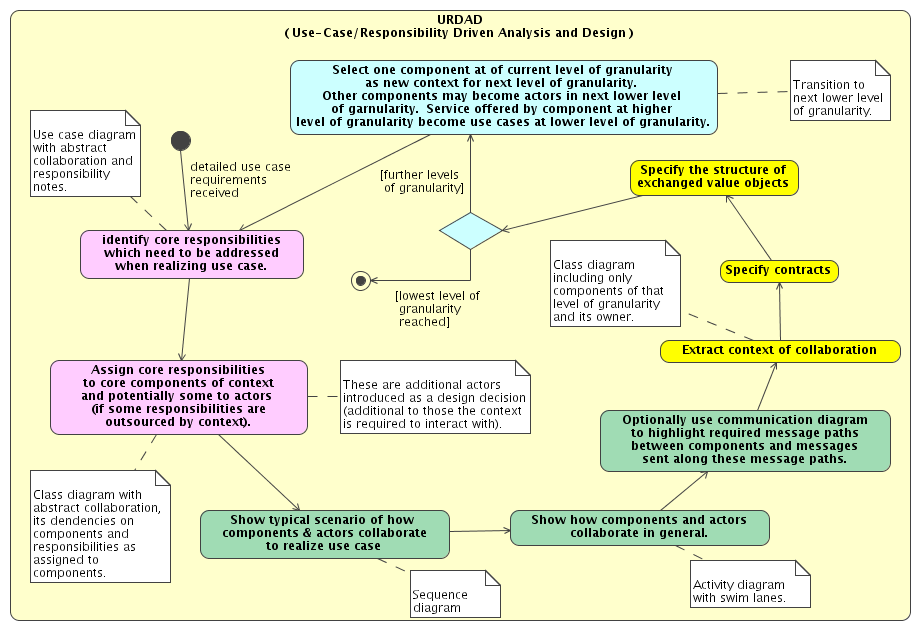
\includegraphics{urdadOverview.png}
    \end{center}
    \caption{Overview of Use-Case/Responsibility Driven Design
        \label{figUrdadOverview}}
\end{figure}

Figure \ref{figUrdadOverview} provides an overview of URDAD. The core steps of an iteration in URDAD are 
\begin{enumerate}
  \item Identify the core responsibilities which need to be addressed when realizing the use case.
  \item Allocate each responsibility to either a component of the current context or an actor.
  \item Specify how these components and actors collaborate to realize the use case.
  \item Project out the context of the collaboration. This is that subset of the static model which at the current level of granularity is required to realize the use case.
  \item Specify for each responsibility the contract they have to realize in the context of the current use case.
  \item Specify the structure of exchanged value objects using class diagrams.
  \item Traverse to the next lower level of granularity by selecting one of the components from the previous iteration as the new context with the services at the previous level of granularity becoming the use cases of this new, lower level of granularity.
	\item Repeat the above steps for the use cases at the next lower level of granularity.
\end{enumerate}
In the following sections these steps will be explained in detail, using the design of a simple mail client as an example.

Note that URDAD is a double-iterative process with 
\begin{enumerate}
  \item {\em use case iterations} ensuring the system is designed iteratively, realizing use case after use case, and
  \item {\em design iterations} taking the design iteratively through lower and lower levels of granularity.
\end{enumerate}

\subsection{Responsibility Identification}
\label{secResponsibilityIdentification}

The first step of URDAD focuses on identifying the responsibilities which need to be addressed when realizing the use case. It is in many respects the most critical and most difficult step. This step fixes the level of granularity for the current design iteration. To this end it is important that the responsibilities identified are at the same level of granularity (or the same level of abstraction). 

\begin{figure}[htb]
    \begin{center}
      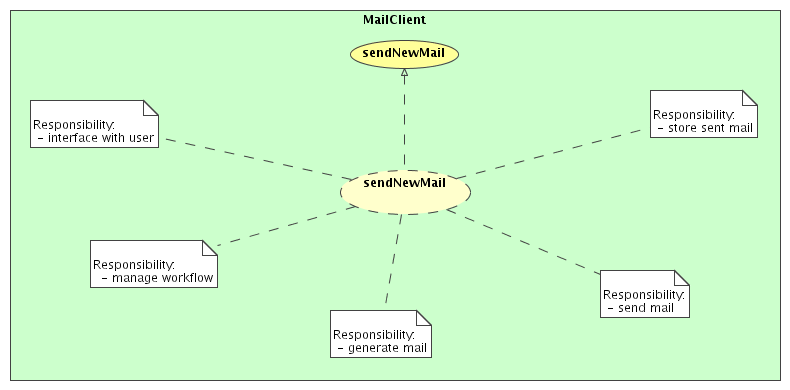
\includegraphics{sendNewMailResponsibilityIdentification.png}
    \end{center}
    \caption{Responsibility identification. \label{figSendNewMailResponsibilityIdentification}}
\end{figure}

Note that URDAD requires that the {\em responsibilities should be identified before identifying system components}. As a second step these responsibilities will be assigned to core system components, ensuring good responsibility localization across system components.

Consider, as an example, a simple mail client. Assume we want to realize the {\em send-new-mail} use case. This use case will be realized through the collaboration of certain system components and potentially some actors. In figure \ref{figSendNewMailResponsibilityIdentification} we identify the responsibilities which need to be addressed when realizing the use case. They include 
\begin{itemize}
  \item the workflow control and user interfacing responsibilities for the current context (the mail client as a whole),
  \item and the functional responsibilities for the mail client including that of generating the e-mail, sending it and storing the sent mail.
\end{itemize}

Responsibilities like that of managing addresses or marshaling the message on to the SMTP protocol are not relevant at this highest level of granularity. The responsibility of selecting addresses for an e-mail will be addressed in the context of creating the mail object and that of marshaling the mail onto the SMTP protocol will be addressed in the context of sending the e-mail. Hence both these responsibilities are lower level responsibilities which will be addressed at a lower level of granularity.

\subsection{Responsibility Allocation}
\label{secResponsibilityAllocation}

The second step of URDAD requires that each responsibility is assigned either to a separate system component or to an actor. URDAD thus enforces the single responsibility principle by design. The objects thus introduced will all be at the same level of granularity as fixed by the responsibilities identified in the first step.

\begin{figure}[htb]
    \begin{center}
      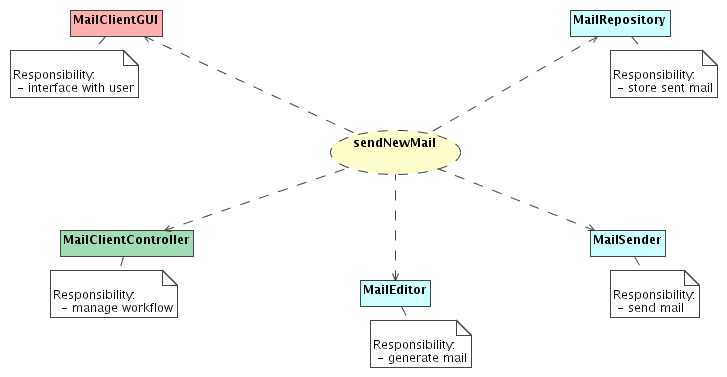
\includegraphics{sendNewMailResponsibilityAllocation.png}
    \end{center}
    \caption{Responsibility allocation. \label{figSendNewMailResponsibilityAllocation}}
\end{figure}

Revisiting our mail client we could potentially assign the responsibilities as illustrated in figure \ref{figSendNewMailResponsibilityAllocation}.

\subsection{Specifying the collaboration}
\label{secCollaboration}

Having 
\begin{enumerate}
  \item identified the responsibilities which need to be addressed when realizing the use case, and
  \item assigned these responsibilities to core system components and external service providers (actors),
\end{enumerate}
we now need to look at how these components and actors collaborate to realize the use case.

Usually one first looks at a particular example (scenario) of realizing the use case. To this end one generally starts with a sequence diagram. Figure�\ref{figSendNewMailSequence} shows an example of such a sequence diagram.

\begin{figure}[htb]
    \begin{center}
      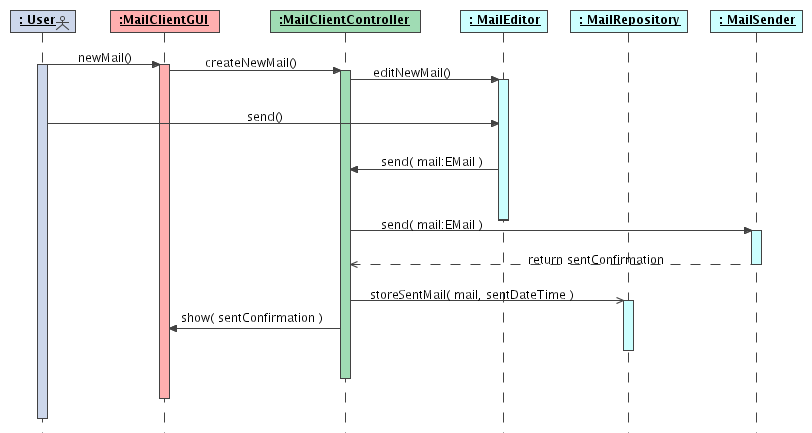
\includegraphics{sendNewMailSequence.png}
    \end{center}
    \caption{A scenario of realizing a use case at a specific level of granularity. \label{figSendNewMailSequence}}
\end{figure}

Note that the only objects participating in the collaboration shown in the sequence diagram are those which address the core responsibilities as identified for this level of granularity.

Once one is comfortable with a particular scenario (often a typical success scenario is chosen), one can look at the collaboration in general. This is commonly documented using a UML activity diagram. In figure \ref{figSendNewMailActivity} we show an activity diagram documenting the general {\em send new mail} collaboration at the current level of granularity as fixed by the initial responsibility identification step.


\begin{figure}[htb]
    \begin{center}
      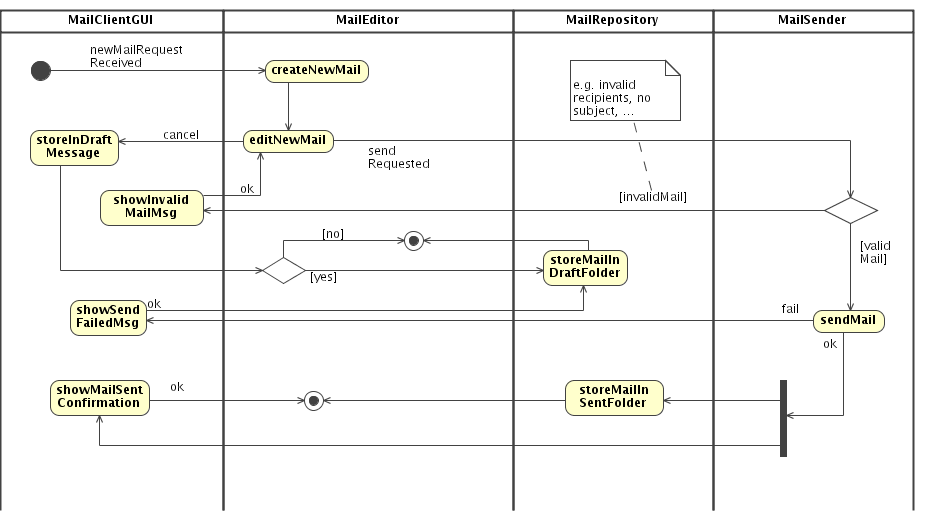
\includegraphics{sendNewMailActivity.png}
    \end{center}
    \caption{The use case collaboration in general. \label{figSendNewMailActivity}}
\end{figure}

Finally, to simplify the transition to the collaboration context, one can use a UML communication diagram. It highlights the required communication paths as well as the service request messages sent along these paths and may contain other information from the static model. URDAD refrains from adding further structural information at this stage. The communication diagram corresponding to the sequence diagram in figure \ref{figSendNewMailSequence} is shown in figure \ref{figSendNewMailCommunicationDiagram}.
 
Note that since URDAD only feeds message path information into communication diagram, the latter contains essentially the same information as the sequence diagram and may be auto-generated from the latter. This step may be (and often is) omitted.

\begin{figure}[htb]
    \begin{center}
      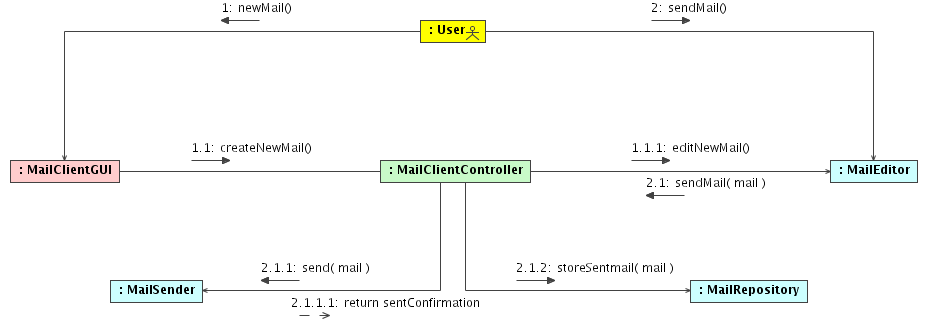
\includegraphics{sendNewMailCommunicationDiagram.png}
    \end{center}
    \caption{Communication diagram simplifying transition to collaboration context. \label{figSendNewMailCommunicationDiagram}}
\end{figure}

\subsection{Projecting out the context of the collaboration}
\label{secCollaborationContext}

The collaboration shows the services the role players request from each other in the context of realizing the use case as well as the message paths required between them. URDAD now generates the context of the collaboration by projecting out the static structure required at the current level of granularity to realize the use case. This is a very simple step and the resultant class diagram is shown in figure \ref{figSendNewMailCollaborationContext}.

\begin{figure}[htb]
    \begin{center}
      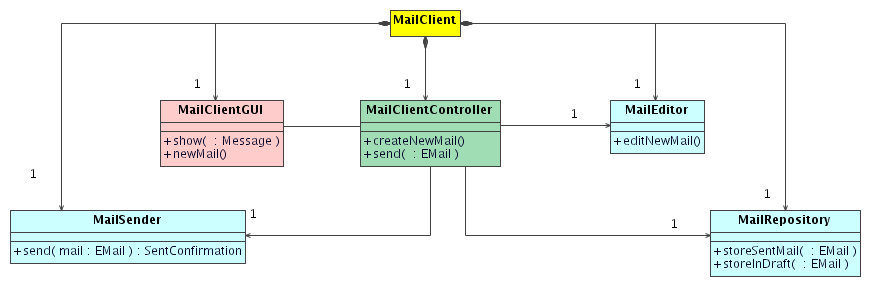
\includegraphics{sendNewMailCollaborationContext.png}
    \end{center}
    \caption{The context of the collaboration. \label{figSendNewMailCollaborationContext}}
\end{figure}

The context of the collaboration is thus that subset of the static model which, at the current level of granularity, is required to realize the use case. The objects from that level of granularity are peers and hence the relationships between them will be associations (client-server) and not aggregation or composition relationships (otherwise the objects would not all be at the same level of granularity). However, some of these are components of the higher level context, filling in composition relationships between layers of granularity.

Note that unlike many other design methodologies (see for example \cite{Ben-Abdallah2004}) which go from the use case model to the static model (often via an object dictionary), URDAD defines the dynamics realizing the use case first. Only then is the required static structure identified. URDAD thus generates minimal structural complexity, i.e. only those structural features which are actually required to realize the use case.

Note also that the objects and classes generated are all at the same level of granularity. They are all either components of the use case context or actors. We have explicitly refrained from introducing any lower level classes at this stage. Instead URDAD provides a simple approach for going over to the next lower level of granularity.

\subsection{Service provider contracts}
\label{secContracts}

Like many other modern design approaches, URDAD is also contract centric. For each component at any level of granularity one first specifies the contract. After all the difference between a class and a component is that the latter realizes a contract as specified by an interface with pre- and post conditions, invariance constraints and quality requirements. Contracts facilitate not only pluggability but also testability -- what would you be testing if there was no contract? 
URDAD requires that tests should be written for contracts (interfaces), not for classes. Any service provider claiming to realize a specific contract should be tested against the test for that contract.

URDAD requires that for each responsibility there should be a contract against which all service providers (components) which realize that responsibility should be tested. The contract may have functional aspects and non-functional aspects. The functional aspects are defined within the standard design-by-contract framework (see \cite{Meyer1991} and \cite{Meyer1992}) by an interface with pre- and post-conditions on the services and, if applicable, invariance constraints on the service provider itself. Contracts are developed from the perspective of the client. They thus resemble the ``signed contracts'' of Andreas Rausch (see \cite{Rausch2002}).

The non-functional aspects may include features like scaleability, usability, reliability, security, and so on. These are typically specified in a quality requirements note.

\subsubsection{Pre-Conditions}

If any of the pre-conditions is not met, the service provider is entitled to refuse the service without breaking the contract. On the other hand, if all preconditions are met, the service provider is obliged to provide the service. Otherwise it is a breach of contract and hence a failure.  For example, for the debit service of an account there may be the pre-condition that there must be sufficient funds in the account. If there are insufficient funds the account
may refuse the service without breaking the contract.

Note that a service provider may experience an internal fault. If that fault is handled and the service provider still provides the service as per contract then no failure occurred.

In software systems service providers use exceptions to notify clients that a requested service is refused due to a pre-condition violation. 

\subsubsection{Post-Conditions}

The post-conditions are the deliverables of the service provider. These include the return value, but may also include service provider state information.

For example, the post-condition of debiting an account may include the requirement that the transaction must have been entered into the account's transaction history.

\subsubsection{Invariance constraints}

These are symmetry rules around the service provider's state. If at any stage (or at least on transactional boundaries) any of the invariance constraints are not met, then the object and hence the system is in an invalid state.

For example, for an account the invariance constraint could be that the sum of all credits minus the sum of all debits must always yield the current balance. If at any stage (at least on transactional boundaries) this symmetry does not hold, then the account and hence the system is in failure.

\subsubsection{Quality requirements}

From design by contract we know that the interface together with the pre- and post-conditions and invariance constraints provide a complete functional requirements specification for a service provider. In addition to the functional requirements, service provider may also need to adhere to certain non-functional (quality) requirements like scaleability, reliability or security requirements. Adding these quality requirements to the functional requirements completes the contract.

For our \verb+MailSender+ component we could require auditability as a non-functional requirement. The latter may be facilitated through logging all send requests together with their completion status.

\subsubsection{Contracts and testing}

Tests should be developed for contracts, not for individual service providers. The tests need to test both the functional, as well as the non-functional aspects of a contract.

During functional testing one tests that, if all preconditions are met, the service is provided such that 
\begin{enumerate}
  \item the client obtains the correct return value,
  \item all post-conditions are met, and
  \item if the invariance constraints were met prior to the service having been requested, that they are still met after the service has been provided.
\end{enumerate}

\subsubsection{Contracts and the Object Constraint Language}

UML enables one to specify the contracts formally in OCL, UML's {\em{Object Constraint Language}}. Doing this facilitates the automatic generation functional and system integrity tests.

\subsubsection{MailSender contract}

Figure�\ref{figContract} shows an informal contract for the \verb+MailSender+ component. It shows the required services together with the pre- and post-conditions for them as well as the non-functional auditability requirement. The contract could be formalized using the OCL.

\begin{figure}[htb]
    \begin{center}
      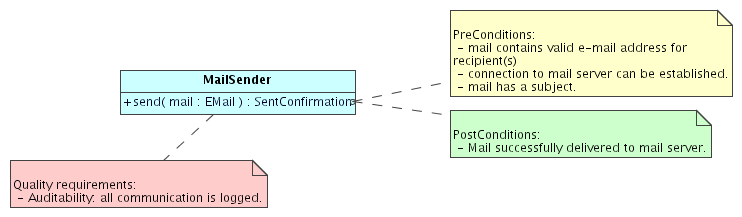
\includegraphics{contract.png}
    \end{center}
    \caption{Contracts are specified for each responsibility and hence for each service provider. \label{figContract}}
\end{figure}

\subsection{Value objects}
\label{secEntityObjects}

One still needs to specify the structure of any object exchanged between system components or between system components and actors, the so-called ``value objects''. If we look at our mail client, then we see that an instance of an \verb+EMail+ is sent from the \verb+MailClientController+ to the \verb+MailSender+ and that the latter returns an instance of a \verb+SentConfirmation+. We need to specify the structure of these value objects. This is naturally done using UML class diagrams.

\begin{figure}[htb]
    \begin{center}
      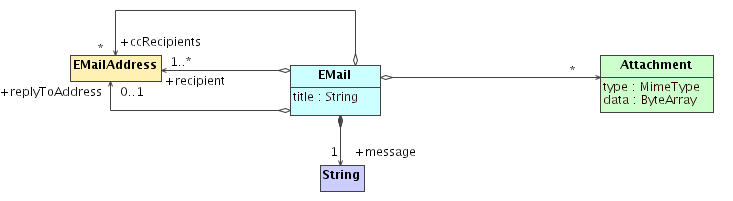
\includegraphics{eMail.png}
    \end{center}
    \caption{Class diagram for the e-mail value object. \label{figEmail}}
\end{figure}

Figure�\ref{figEmail} shows a simplified class diagram for the e-mail value object exchanged between the \verb+MailEditor+, \verb+MailClientController+ and \verb+MailSender+.

\subsection{Transition to the next level of granularity}
\label{secNextLevelOfGranularity}

In order to go over to the next level of granularity, one selects one of the components from the current level of granularity as the context for the next level of granularity. Its services at the current level of granularity will become the use cases of the next level of granularity. Those components which interface with that object at the current level of granularity will become the actors. For example, if we select the \verb+MailSender+ as our new context, the corresponding use case diagram would be given by figure \ref{figMailSenderUseCase}, i.e.\ the \verb+MailSender+ is used by the \verb+MailClientController+ to send e-mails.

\begin{figure}[htb]
    \begin{center}
      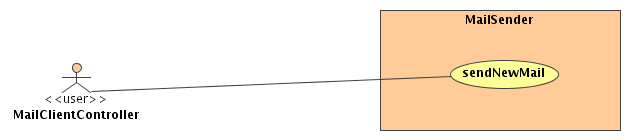
\includegraphics{mailSenderUseCase.png}
    \end{center}
    \caption{Use case diagram for a component at the next lower level of granularity. \label{figMailSenderUseCase}}
\end{figure}

Of course the object may choose to realize the use case in a way which makes use of further actors. This should, however, be responsibility driven. We thus first identify the responsibilities at this new, lower level of granularity and before assigning them to components and/or actors of this lower level object as shown in figure�\ref{figSendMailResponsibilityIdentification}.

\begin{figure}[htb]
    \begin{center}
      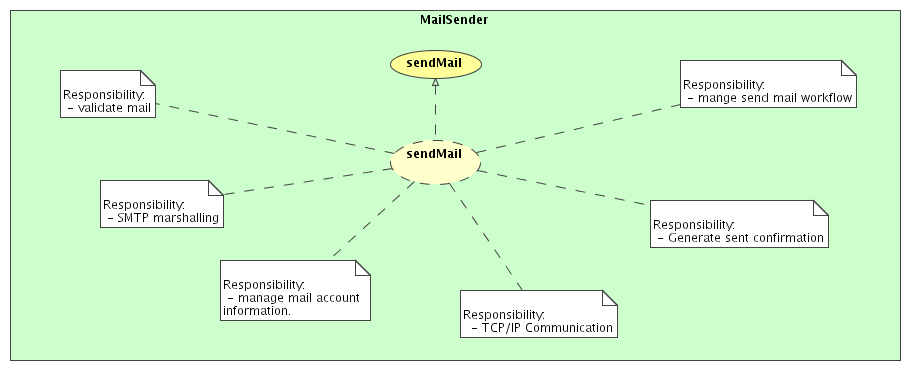
\includegraphics{sendMailResponsibilityIdentification.png}
    \end{center}
    \caption{Responsibility identification at next lower level of granularity. \label{figSendMailResponsibilityIdentification}}
\end{figure}

Each responsibility is, once again, assigned to either a component of this lower level component (this is where the composition relationships are identified) or an actor. This is shown in figure�\ref{figSendMailResponsibilityAllocation}.

\begin{figure}[htb]
    \begin{center}
      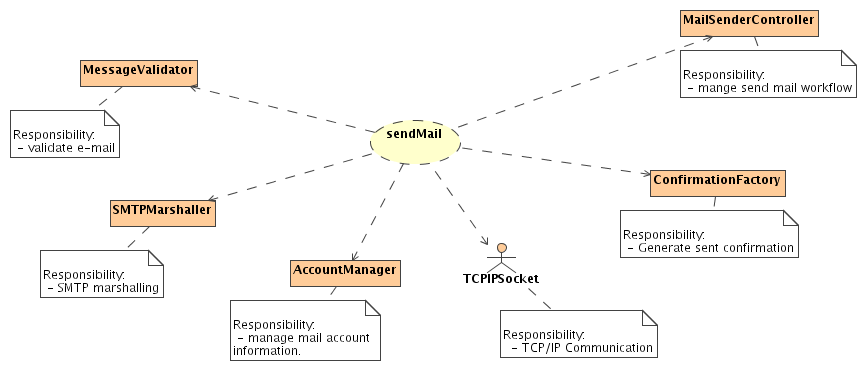
\includegraphics{sendMailResponsibilityAllocation.png}
    \end{center}
    \caption{Responsibility allocation at next lower level of granularity. \label{figSendMailResponsibilityAllocation}}
\end{figure}

Note that we have a workflow controller at each level of granularity taking over the responsibility of managing the workflow for the use case at that level of granularity. Similarly, if the user interfaces directly with the lower level object (as, for example, the \verb+MailEditor+ would), then there would also be the responsibility of interfacing with the user.

URDAD is thus an iterative design process which projects out one level of granularity after another. Typically one will require between 2 and 4 levels of granularity depending on the complexity of the system.

\section{Summary and conclusions}
\label{secSummary}

URDAD provides a simple algorithm for designing a use case realization. It projects out different levels of granularity. At each level of granularity one starts with responsibility identification followed by responsibility allocation. Once one has established the objects which take care of the responsibilities which need to be addressed when realizing a use case, one specifies how they collaborate. From the collaboration one can project out the collaboration context which is that subset of the static model which, at the current level of granularity, is required to realize the use case. URDAD then provides a simple mechanism for going from the current level of granularity to the next lower level of granularity. This is done by selecting one of the components from the higher level of granularity as new context. Its services at the higher level of granularity become the use cases at the lower level of granularity. Some of the components of the previous level of granularity may become actors at this lower level of granularity. The process continues symmetrically by identifying and assigning responsibilities at the new lower level of granularity to components of the new context and external service providers (actors). The collaboration realizing the lower level use cases project out the static model at this lower level of granularity.

URDAD encourages {\em ``good design''} by  generating clean layers of granularity with minimal structural complexity,
enforcing responsibility localization and contracts across system components.

Finally, URDAD provides a design process which follows the spirit of OMG's Model Driven Architecture (MDA) by generating a platform independent model (PIM). The PIM is then mapped onto some choice of architecture and technologies resulting in the platform specific model (PSM) which is ultimately mapped onto a realization resulting in the Enterprise Deployment Model (EDM).

\begin{thebibliography}{XXXXX}
\bibitem[Ben-Abdallah2004]{Ben-Abdallah2004} H.\ Ben-Abdallah, N.\ Bouassida, F.\ Gargouri and A.\ Ben-Hamadou:
   A UML Based Framework Design Method, Journal of Object Technology, 3 (8), 2004.

\bibitem[Frankel2003]{Frankel2003} David S. Frankel, Model Driven Architecture: Applying MDA to enterprise computing, John Wiley \& Sons, 2003.

\bibitem[Meyer1991]{Meyer1991} Bertrand Meyer: Design by Contract, Prentice Hall, 1991.


\bibitem[Meyer1992]{Meyer1992} Bertrand Meyer: Applying Design by Contract, Computer (IEEE), 25 (10), 1992, 40-51.

\bibitem[Rausch2002]{Rausch2002} Andreas Rausch: Design by Contract + ComponentWare = Design by Signed Contract,
   Journal of Object Technology, 1 (3), 2002.

\bibitem[Rosen1999]{Rosen1999} Doug Rosenberg et Kendall Scott: Use Case Driven Object Modeling with UML: A Practical Approach, Addison-Wesley Professional, 1999.

\bibitem[Wirfs2002]{Wirfs2002} Rebecca Wirfs-Brock et Alan McKean, Object Design: Roles, Responsibilities and Collaborations, Addison Wesley Professional, 2002.

\bibitem[Wirfs1989]{Wirfs1989}Rebecca Wirfs-Brock and Brian Wilkerson: Object-Oriented Design: 
    A Responsibility-Driven Approach, OOPSLA '89 Proceedings, 1-6 October 1989, pp. 71-75

\bibitem[Wirfs1990]{Wirfs1990} Rebecca Wirfs-Brock, Brian Wilkerson, and Lauren Wiener: Designing Object-Oriented Software, Prentice Hall, 1990.
\end{thebibliography}


% This command starts the ``About the Authors'' section.
\abouttheauthors

\abouttheauthor[Fritz]{Fritz Solms}{ has a PhD in Theoretical Physics from
the University of Pretoria. He is a founding member of Solms Training and
Consulting and has been active in research in software development, business
process design and organizational architecture.
He can be reached at
\maillink{fritz@solms.co.za}. 
See also \htmllink{http://www.solms.co.za}.}

\end{document}
